\documentclass[aspectratio=169]{beamer}
%[handout]

\usetheme[progressbar=frametitle]{metropolis}
\usepackage{appendixnumberbeamer}

\usepackage[utf8]{inputenc}
\usepackage[T1]{fontenc}

\usepackage[brazil]{babel}
\usepackage[outputdir=..]{minted}
\usepackage{xcolor}
\usepackage{soul} % strikethrough
\usepackage{advdate}
\usepackage{graphicx}
\graphicspath{{figs/}}
\usepackage{graphbox}

\usepackage[ampersand]{easylist}

\usepackage{multirow}
\usepackage{multicol}
\usepackage{subcaption}

\usepackage{pgf,tikz}
\usetikzlibrary{shapes,arrows,positioning}
\usetikzlibrary{circuits.logic.US}
\usetikzlibrary{matrix,calc}

\usepackage{karnaugh-map}

\usepackage{pgfpages}
\setbeameroption{hide notes} % Only slides
% \setbeameroption{show only notes} % Only notes
% \setbeameroption{show notes on second screen=right} % Both

% \graphicspath{{../figs/}}

\definecolor{bgc}{rgb}{0.95,0.9,0.95}
\definecolor{links}{HTML}{2A7F7F}
\hypersetup{colorlinks,linkcolor=,urlcolor=links}

\newminted{verilog}{fontsize=\scriptsize, 
    linenos,
    numbersep=8pt,
    bgcolor=bgc,
    tabsize=4,
    framesep=3mm} 
    %frame=lines,

\newcommand{\verilog}[1]{\verilogf{#1}{\footnotesize}}

\newcommand{\verilogf}[2]{\inputminted[fontsize=#2, 
    linenos,
    tabsize=2,
    numbersep=4pt,
    bgcolor=bgc,
    framesep=3mm]{verilog}{../codes/#1.v}
}

\newminted{nasm}{fontsize=\scriptsize, 
		   linenos,
		   numbersep=8pt,
           bgcolor=bgc,
		   framesep=3mm} 

\usepackage{booktabs}
\usepackage[scale=2]{ccicons}

\usepackage{pgfplots}
\usepgfplotslibrary{dateplot}

\usepackage{hyperref}


\usepackage{xspace}
\newcommand{\themename}{\textbf{\textsc{metropolis}}\xspace}



\usepackage{pifont}% http://ctan.org/pkg/pifont
\newcommand{\cmark}{\ding{51}}%
\newcommand{\xmark}{\ding{55}}%

% \tiny	
% \scriptsize
% \footnotesize
% \small	
% \normalsize	
% \large	
% \Large	
% \LARGE	
% \huge	
% \Huge	



\newminted{python}{fontsize=\scriptsize, 
		   linenos,
		   breaklines,
		   numbersep=8pt,
           tabsize=2,
		   framesep=3mm} 
		   
\newminted{verilog}{fontsize=\scriptsize, 
		   linenos,
		   breaklines,
		   numbersep=8pt,
           tabsize=2,
		   framesep=3mm} 
		   




\definecolor{bgc}{rgb}{0.95,0.9,0.95}
\definecolor{links}{HTML}{2A7F7F}
\hypersetup{colorlinks,linkcolor=,urlcolor=links}


% \usepackage[style=apa]{biblatex}
% \addbibresource{mm.bib}


% \author{\large Prof. Ricardo Menotti (\href{mailto:menotti@ufscar.br}{menotti@ufscar.br})}

\newcommand{\newauthor}[2]{
  \parbox{0.50\textwidth}{
    \texorpdfstring
      {
        \centering
        \small #1 \newline
        {\scriptsize{\urlstyle{same}\href{mailto:#2}{#2}\urlstyle{tt}}}
      }
      {#1} \newline
  }
}

\author{
  \newauthor{Prof. Ricardo Menotti}{menotti@ufscar.br}
\and \newauthor{Prof. Luciano de Oliveira Neris}{lneris@ufscar.br}  
%\and \newauthor{Prof. Artino Quintino da Silva Filho}{artino@ufscar.br}
% \and \newauthor{Prof. Maurício Figueiredo}{mauricio@ufscar.br}
% \and \newauthor{Prof. Edilson Kato}{kato@ufscar.br}
% \and \newauthor{Prof. Roberto Inoue}{rsinoue@ufscar.br}
}

\date{Atualizado em: \today}

\institute{\large \textbf{Departamento de Computação} \\
Centro de Ciências Exatas e de Tecnologia \\
Universidade Federal de São Carlos}

\title{Lógica Digital (1001351)}

\titlegraphic{\hfill
\includegraphics[height=1.5cm]{LogoUfscar}}



\subtitle{Introdução} % 

\begin{document}

\begin{frame}
	\titlepage
\end{frame} 

% \begin{frame}{Conteúdo}
% 	\tableofcontents
% \end{frame}

\section{Introdução} %%%%%%%

\begin{frame}{\insertsection} 
	\begin{itemize}
		\item Os circuitos lógicos que veremos deste curso estão presentes nos computadores e em quase todos os aparelhos eletrônicos que conhecemos; 
		\item Entender como eles funcionam é fundamental para as carreiras de computação em geral; 
		\item Nós vamos começar com circuitos simples, mas usando a metodologia adotada na indústria;
		\item Circuitos lógicos são implementados usando transistors (integrados) e podem contar até bilhões deles;
		\item Entender os blocos básicos é simples, mas entender sistemas grandes só será possível se aprendermos as técnicas de projeto adotadas na indústria. 
    \end{itemize}
\end{frame}

\section{Hardware digital}

\begin{frame}{\insertsection}
	\begin{itemize}
        \item O nome \textit{digital} deriva da forma em que a informação é representada, o que será visto logo a seguir; 
        \item Até a década de 60 os circuitos eram construidos com componentes grandes, tais como resistores e transistores, usados separadamente; 
        \item O advento dos circuitos integrados permitiu acoplar um certo número de transistores, e consequentemente um circuito inteiro, em um único chip.
    \end{itemize}
\end{frame}

\begin{frame}{\insertsection} 
    \begin{columns}
        \begin{column}{0.40\textwidth}
            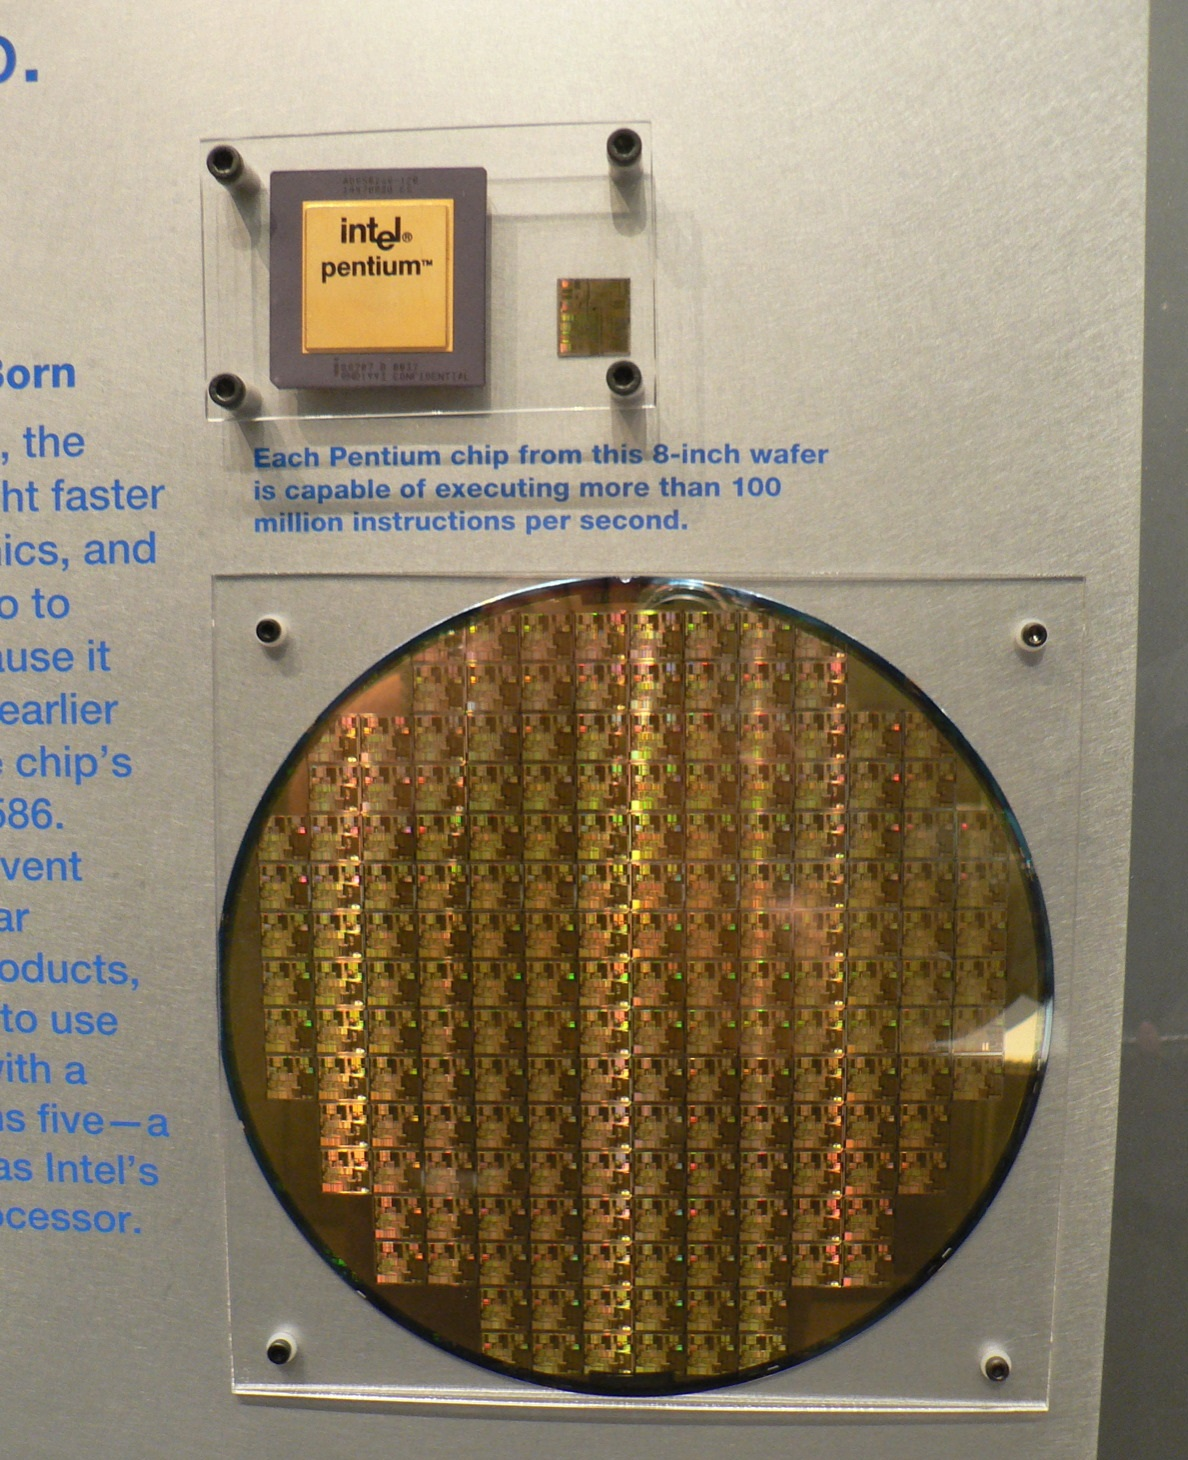
\includegraphics[width=\textwidth]{Wafer_with_Pentium_chips}
        \end{column}
        \begin{column}{0.60\textwidth}
            \centering \textit{``Cada chip do Pentium nesta bolacha de silício de 8 polegadas é capaz de executar mais de 100 milhões de instruções por segundo.''}
        \end{column}
    \end{columns}
\end{frame}

\begin{frame}{Lei de Moore (1965)}
    \centering
    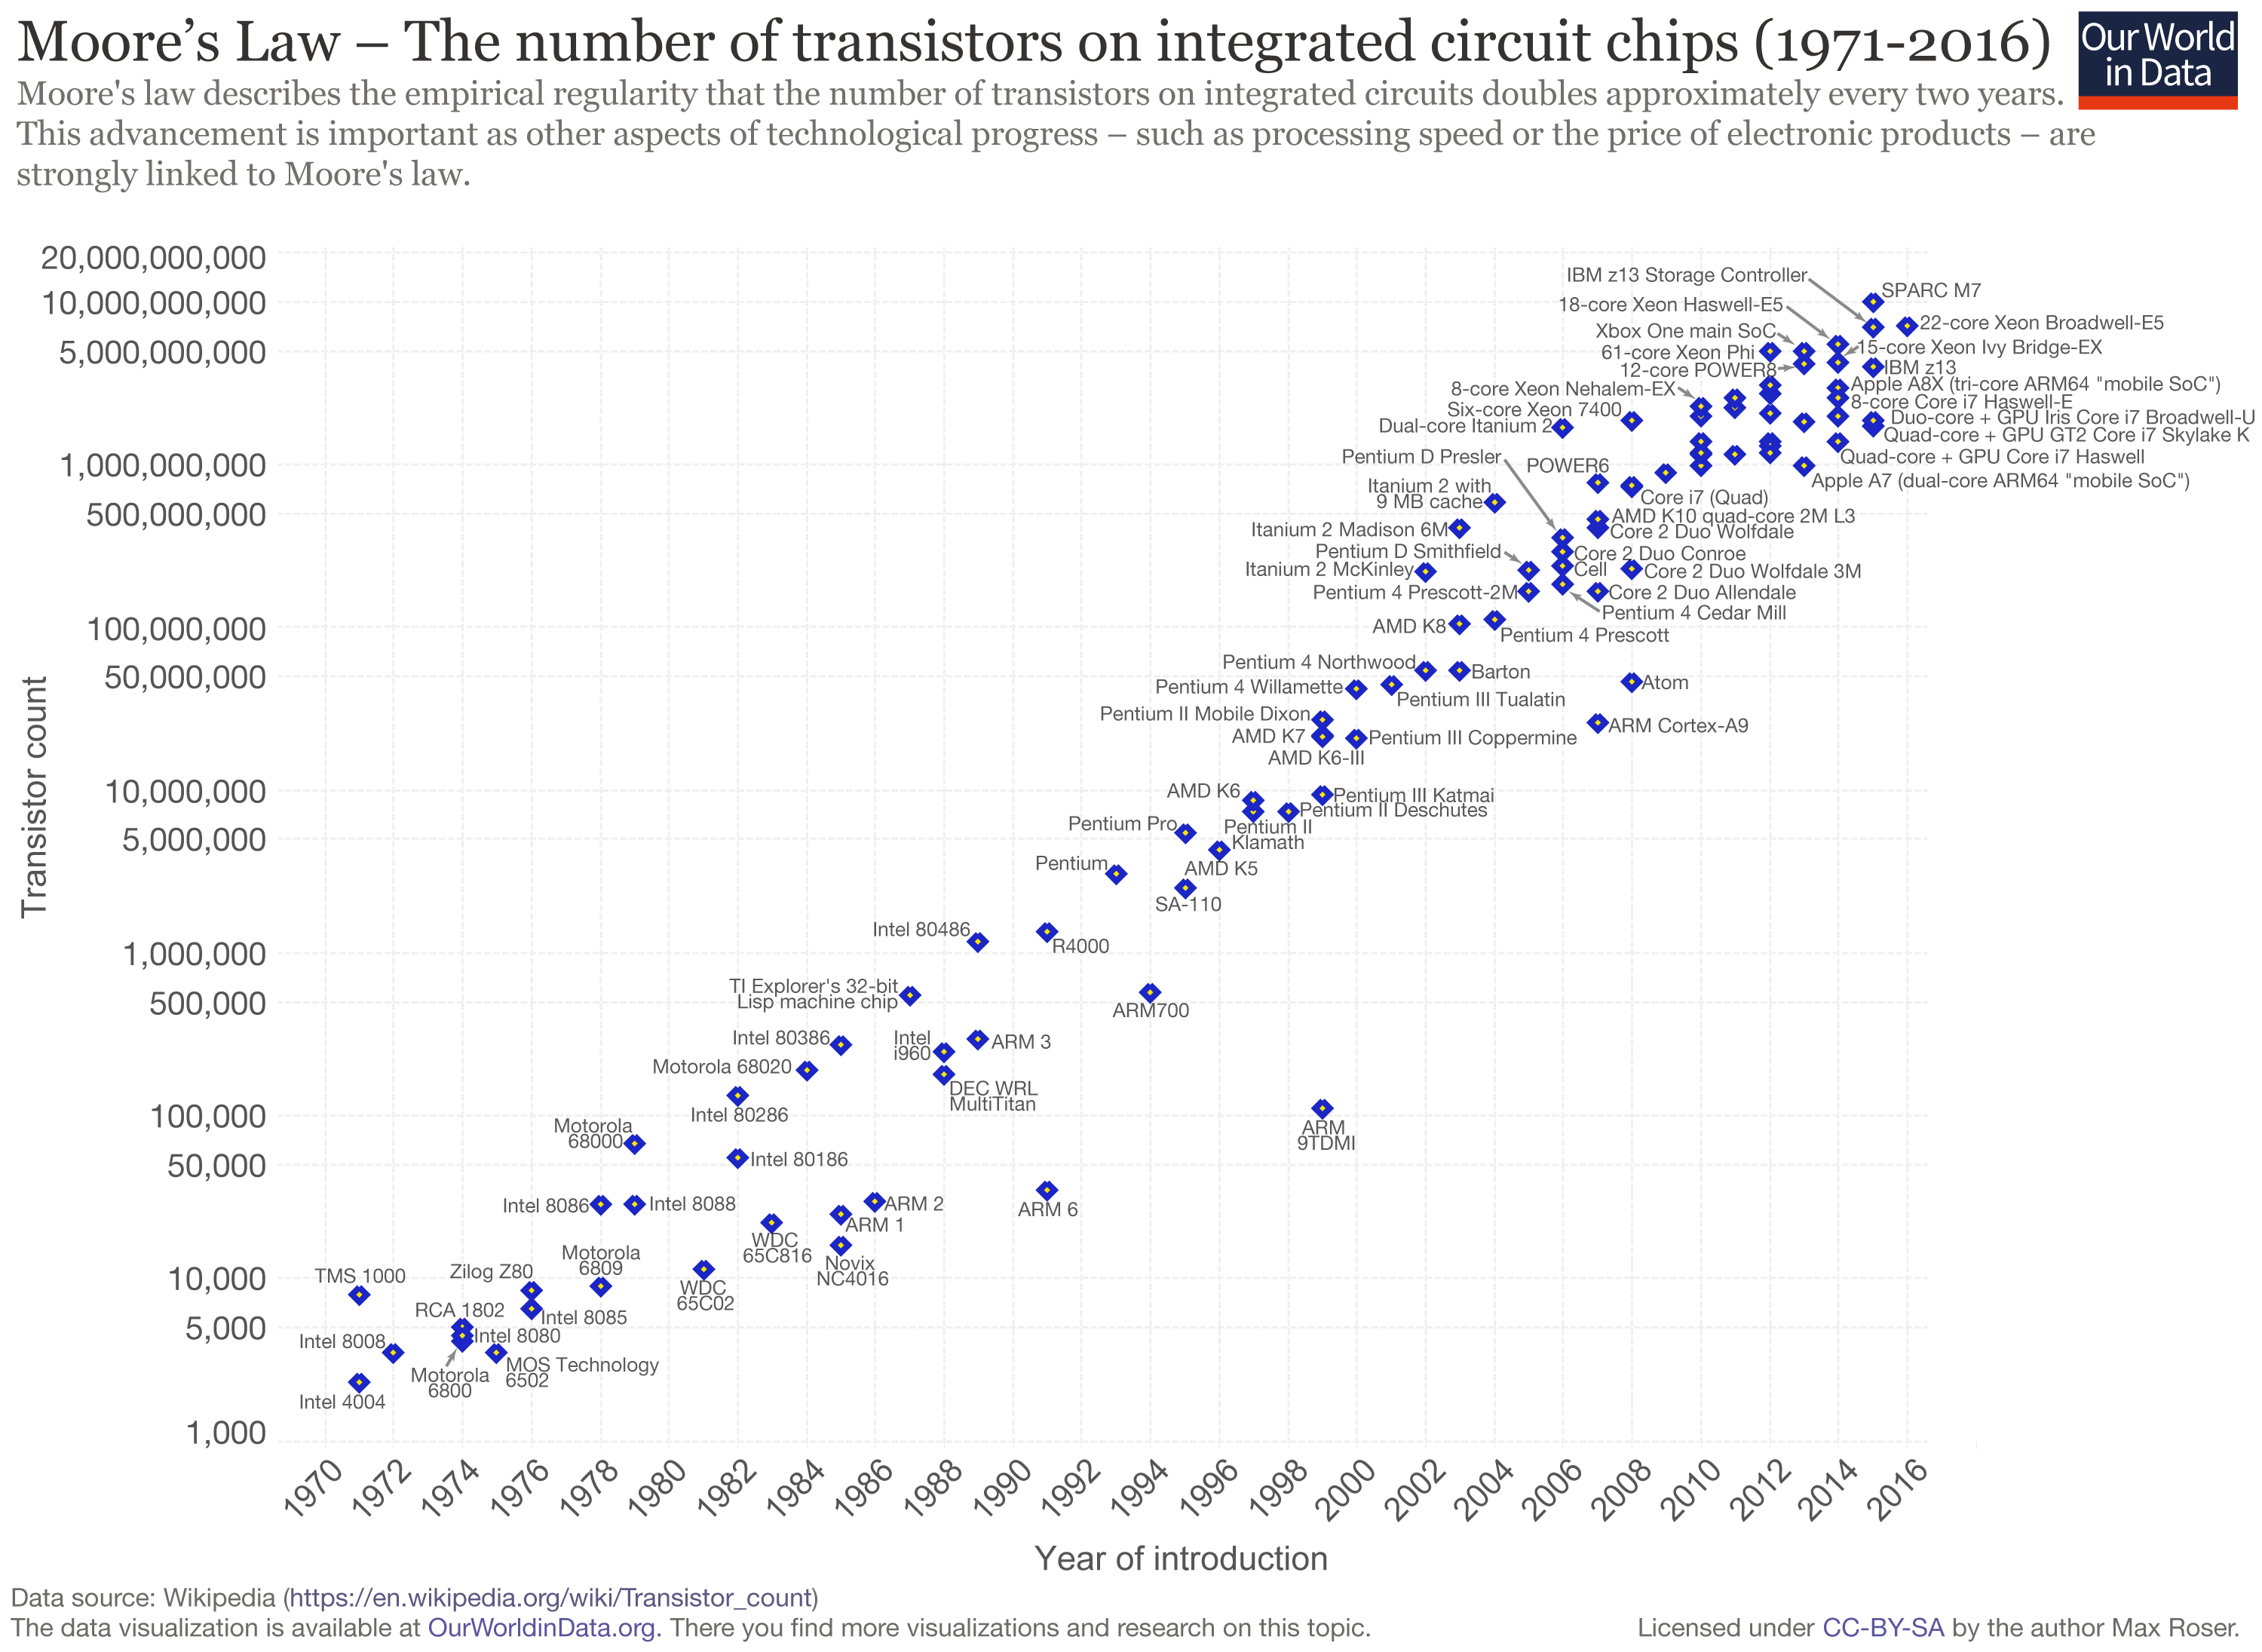
\includegraphics[height=\textheight]{Moore}
\end{frame}

\begin{frame}{Standard Chips} 
    \begin{columns}
        \begin{column}{0.60\textwidth}
            \begin{itemize}
                \item Disponíveis para realizar funções comuns;
                \item Agrupados e conectados para construir um circuito;
                \item Muito usados até a década de 80, mas consomem muito espaço na placa;
                \item Possuem funcionalidades fixas, ou seja, não podem ser mudadas após a fabricação. 
            \end{itemize}
        \end{column}
        \begin{column}{0.40\textwidth}
            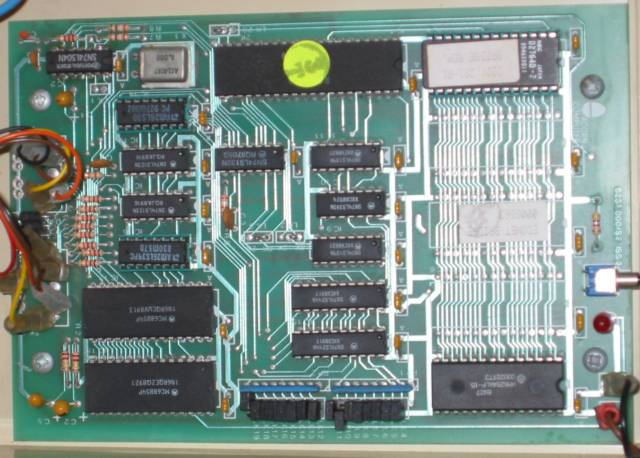
\includegraphics[angle=90,height=\textheight]{Econet}
        \end{column}        
    \end{columns}
\end{frame}

\begin{frame}{\textit{Field-Programmable Gate Array (FPGA)}} 
    \begin{columns}
        \begin{column}{0.340\textwidth}
            \vspace{1cm}
            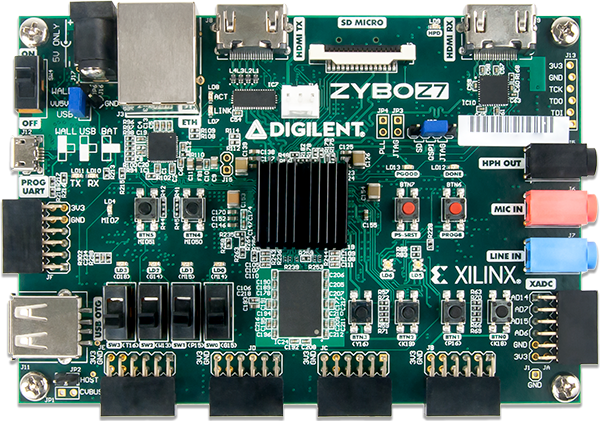
\includegraphics[angle=90,width=\textwidth]{zybo-z7-20}
        \end{column}            \begin{column}{0.60\textwidth}
            \begin{itemize}
                \item \textit{Programmable Logic Devices (PLDs);}
                \item \textit{Field-Programmable Gate Arrays (FPGA);}
                \item Veremos com detalhes mais adiante...
            \end{itemize}
            \vspace{1cm}
            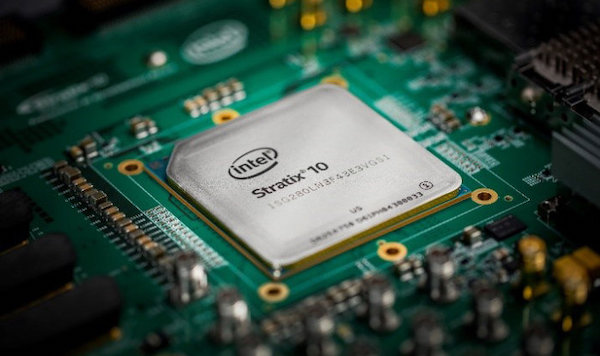
\includegraphics[width=.45\textwidth]{Stratix10} 
            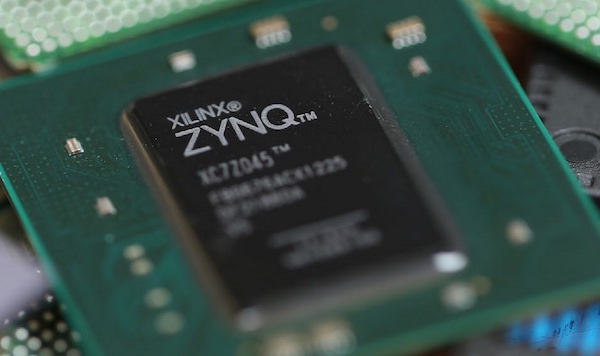
\includegraphics[width=.45\textwidth]{Zynq}
        \end{column}
    \end{columns}
\end{frame}

\begin{frame}{\textit{Application-Specific Integrated Circuit (ASIC)}}
    \begin{itemize}
        \item FPGAs permitem implementar praticamente qualquer circuito, mas têm algumas desvantagens:
        \begin{itemize}
            \item custam mais caro;
            \item ocupam mais espaço; e 
            \item possuem desempenho limitado;
        \end{itemize}  
        \item Para atingir melhores resultados é possível criar um chip do zero:
        \begin{itemize}
            \item \textit{[semi-]custom design};
        \end{itemize}
        \item \textit{Application-Specific Integrated Circuit (ASIC)}
    \end{itemize}
\end{frame}

\begin{frame}{\textit{Application-Specific Integrated Circuit (ASIC)}}
    \begin{itemize}
        \item Podem ser otimizados para um determinada tarefa, apresentando melhor desempenho;
        \item Seu custo é alto, mas se fabricado em grandes quantidades oferece a melhor relação custo-benefício;
        \item Uma desvantagem  é que a fabricação de um chip personalizado muitas vezes leva uma quantidade considerável de tempo, na ordem dos meses.
    \end{itemize}
\end{frame}

\begin{frame}{\insertsection}
    \centering 
    \tikzstyle{decision} = [diamond, draw, fill=red!20, text width=4.5em, text badly centered, node distance=2.3cm, inner sep=0pt]
    \tikzstyle{block} = [rectangle, draw, fill=red!20, text width=10em, text centered, rounded corners, minimum height=2em]
    \tikzstyle{line} = [draw, -latex']
    \tikzstyle{cloud} = [draw, ellipse,fill=red!20, node distance=3cm,
    minimum height=2em]
\resizebox{0.35\textwidth}{!}{%
\begin{tikzpicture}[node distance = 1.3cm, auto]
    \node [cloud] (init) {Produto requerido};
    \node [block, below of=init] (specs) {Definir espeficicação};
    \node [block, below of=specs] (design) {Projeto inicial};
    \node [block, below of=design] (sim) {Simulação};
    \node [block, right=1cm of sim] (redesign) {Reprojeto};
    \node [decision, below of=sim] (right) {Projeto correto?};
    \node [block, below=0.7cm of right] (proto) {Prototipação};
    \node [block, below of=proto] (test) {Testes};
    \node [block, right=1cm of proto] (corec) {Correções};
    \node [decision, below of=corec] (minor) {Erros menores?};
    \node [decision, below=0.7cm of test] (meets) {Cumpre especificação?};
    \node [cloud, below=0.3cm of meets] (finish) {Produto finalizado};
    \path [line] (init) -- (specs);
    \path [line] (specs) -- (design);
    \path [line] (design) -- (sim);
    \path [line] (sim) -- (right);
    \path [line] (redesign) -- (sim);
    \path [line] (right) -| (redesign) node[near start,above] {não};
    \path [line] (right) -- (proto) node[near start,right] {sim};
    \path [line] (proto) -- (test);
    \path [line] (test) -- (meets);
    \path [line] (corec) -- (proto);
    \path [line] (minor) -- (corec) node[near start,right] {sim};
    \path [line] (meets) -| (minor) node[near start,above] {não};
    \path [line] (meets) -- (finish) node[near start,right] {sim};
    \path [line] (minor.east) -- node[near start,above] {não} ++(2,0)  -- ++(0,6.95) --  (redesign.east);
\end{tikzpicture}}
\end{frame}




\section{Bibliografia} %%%%%%%


\begin{frame}[allowframebreaks]{\insertsection} 
	\begin{itemize}
		\item Básica
		\begin{itemize}
			\item \href{https://www.google.com.br/search?q=filetype\%3Apdf+Fundamentals+of+Digital+Logic+with+Verilog+Design+&oq=filetype\%3Apdf}{Brown, S. \& Vranesic, Z. - Fundamentals of Digital Logic with Verilog Design, 3rd Ed., Mc Graw Hill, 2009}
			\item \href{https://www.sciencedirect.com/science/book/9780123944245}{D. M. Harris \& S. L. Harris - Digital Design and Computer Architecture 2nd Ed., Elsevier, 2012}
		\end{itemize}
		\item Complementar
		\begin{itemize}
			\item \href{https://irds.ieee.org/}{International Roadmap for Devices and Systems}
		\end{itemize}
	\end{itemize}
\end{frame}


\begin{frame}
	\titlepage
\end{frame} 

\end{document}